\documentclass[]{final_report}
\usepackage{graphicx}
\usepackage{hyperref}
\usepackage[normalem]{ulem}
\usepackage{amsmath}
\usepackage{csvsimple}
\usepackage{float}
\usepackage[]{algorithm2e}
\usepackage[noend]{algpseudocode}
\usepackage{url}
\usepackage{listings}             % Include the listings-package
\usepackage{enumerate}
\usepackage{cite}



\RestyleAlgo{boxruled}
\lstset{language=Python}
\newcommand{\myparagraph}[1]{\paragraph{#1}\mbox{}\\}

%%%%%%%%%%%%%%%%%%%%%%
%%% Project details
%%%%%%%%%%%%%%%%%%%%%%
\def\studentname{Kamil Smuga}
\def\projecttitle{An approach for Continuous Capacity Planning in Cloud Environments with an Uptime-based Pricing Model}
\def\supervisorname{Prof. Liam Murphy}
\def\moderatorname{Christina Thorpe}

\begin{document}

\maketitle
\tableofcontents\pdfbookmark[0]{Table of Contents}{toc}\newpage
\listoffigures\newpage
\par{\textbf{List of tables}}

%%%%
%The most important parts of your thesis are: abstract, introduction, conclusion and
%references. These are what get read first and make that vital initial impression.
%%%
%%%
%One of first things your examiners will look at is your literature review. If they see a
%good number of journal papers, a swathe of conference papers, a few recent workshop
%papers and not too many web sites, they’ll already be impressed.
%%%
%%%%%%%%%%%%%%%%%%%%%%
%%% ABSTRACT 
%%%%%%%%%%%%%%%%%%%%%%

\begin{abstract}

\emph{ /* To be revised. */} \par
\textsl{New Infrastructure as a Service solutions are becoming available with a growing number of supported pricing models. More often than not, a hosted Cloud environment is used to design and build an infrastructure for a product. The recent availability of different pricing schemes based on resource utilization and uptime reveals new challenges in already unpredictable capacity planning process. There is a choice between ad-hoc provisioning and upfront payments with reduced hourly rates. Reserved instances charged upfront are categorized into three groups: light, medium and heavy. Which one is better for a given utilization model? When exactly does one pricing scheme becomes more cost effective? Determining which machine type is better for a given utilization model, or at which point the cost effectiveness of a pricing scheme changes, is vital for the companies subscribing to the IaaS. }

\end{abstract}
\newpage

%%%%%%%%%%%%%%%%%%%%%%
%%% INTRODUCTION 
%%%%%%%%%%%%%%%%%%%%%%

\chapter{Introduction}

\emph{ /* Type of the project: The 'Big Idea' / proof by construction. */}

\section{Description of the problem}

\section{Motivation for solving the problem}

\section{Objectives}
This work aims to design an algorithm that answer IaaS consumer's price optimality questions and help to make adjustments based on uptime based charging per machine. 

\section{Related work}

\section{Challenges}

\section{Description of methodology}
Modelling and experimentation

\section{Structure of the Thesis}
\textbf{Background}. This section will outline the background information related to IaaS consumer challenges related to understanding the whole picture for price optimality of rented infrastructure. \par
\textbf{Design}. This section explains design and environment conditions for the algorithm to be useful. \par
\textbf{Implementation}. This section explains algorithm implementation details and data analytics software that was used - Apache Spark\footnote{\url{https://spark.apache.org}}. \par
\textbf{Evaluation}. The proposed algorithmic approach is applied to Google Trace data~\cite{clusterdata:Reiss2011}. \par
\textbf{Conclusion and Future Work}. The completed data analysis is discussed. Further work related to algorithm improvements, automation and lessons learned are presented. 
 
\newpage

%%%%%%%%%%%%%%%%%%%%%%
%%% BACKGROUND 
%%%%%%%%%%%%%%%%%%%%%%

\chapter{Background}

\section{The Problem Domain}
\emph{/* Description of IaaS world - providers and consumers. */}
\subsection{IaaS consumer point of view}
\subsection{IaaS provider uptime-based pricing schemes}

\section{Motivation}
\emph{ /* Description of the problem - cloud-based company runs a mix of software services (real-time streaming, batch, web and database servers) on common hardware. How do they know whether provisioned VMs run in the most optimal configuration? */ }

\section{Literature review}
\emph{/* Haven't found anything that would tackle this specific problem so far. Might mention the most research is done from IaaS provider perspective? This includes resource scheduling. My work can lead to cost-aware scheduler research */}

%good number of journal papers, a swathe of conference papers, a few recent workshop
%papers and not too many web sites


%%%%%%%%%%%%%%%%%%%%%%
%%% DESIGN 
%%%%%%%%%%%%%%%%%%%%%%

\chapter{Design and Implementation}

\section{Taxonomy}

\subsection{Upfront cost}

Investment in compute resources comes with upfront cost. In case of physical machine it is hardware or lease cost. For virtual resources, IaaS providers offer per hour discounts for upfront charged schemes. \par
Upfront cost is considered to be one time payment and will be represented by \textit{u}. 

\subsection{Cost per hour}

Cost per hour represents a total cost of running a single machine divided by number of hours in calendar year. Aggregated cost is relatively easy to calculate in rented, virtualized environments. IaaS providers usually charge an X amount per hour. It might vary based on total uptime per month or pricing scheme. This number will be considered as a partial cost per hour and defined as \textit{pcph}. \par
Cost per hour will be defined as \textit{cph}. It includes upfront cost and IaaS provider per hour charges. It is defined as a function of hours of utilization per day.  

\begin{equation}
\label{eq:cph}
cph(h) = \frac{u + \sum_{i=1}^{366} pcph \times h}{365 \times h}
\end{equation}

\subsection{Intersection points between pricing schemes}

TO BE REWRITTEN!

Cost per hour is calculated for each of available pricing schemes. Single result represents a matrix of hours per day and \textit{cph}. Graphical representation of results produces a graph similar to Figure~\ref{fig:cc2_8xlarge}. \par 
This representation allows to notice pricing trends. In the example below, price drops exponentially for around first 5 hours of usage and nearly stabilizes afterward. Light is the cheapest option for around 15 hours per day usage. This is better visible on Figure~\ref{fig:cph_cc2_8xlarge_zoom}. After 15 hours, it is better to invest in the Heavy utilization scheme. This is the point that will be called \textit{an intersection point} between 2 pricing schemes and noted as \textit{ip(scheme1, scheme2)}. \par
For the example below, cc2.8xlarge instance's intersection point between Light and Heavy schemes is \textit{ip(light, heavy) = 16}.

\begin{figure}[H]
	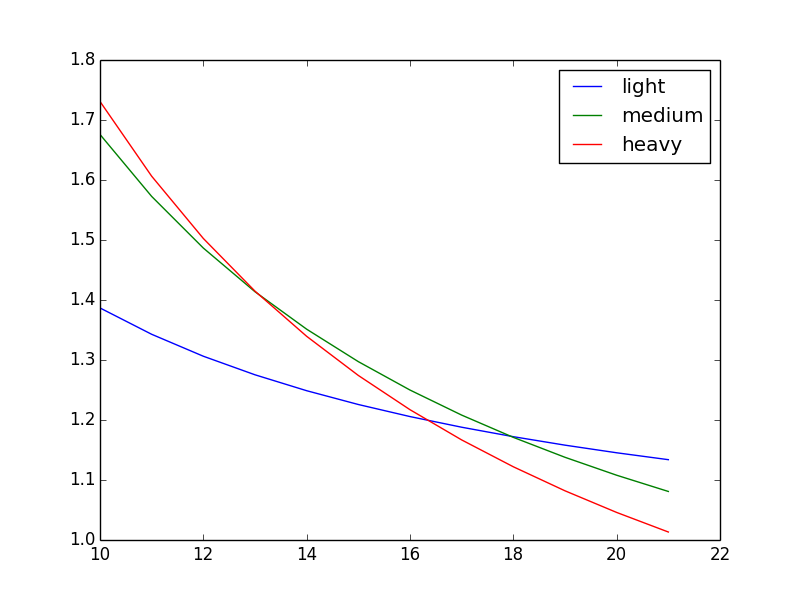
\includegraphics[width=\linewidth]{figures/cph_cc2_8xlarge_zoom}
	\caption{Zoomed \textit{cph} results for Amazon AWS cc2.8xlarge reserved instance rented for 1 year~\cite{AWS:light}~\cite{AWS:medium}~\cite{AWS:heavy}}
	\label{fig:cph_cc2_8xlarge_zoom}
\end{figure}


\section{Algorithm}

\subsection{Prerequisites} 

In order to make data-driven analysis and suggestions for optimization, we need data. The below list of metrics was compiled based on algorithm needs to answer critical questions regarding the state of infrastructure deployment. The list is suitable to guarantee performance SLOs only for compute nodes. Machines with significant I/O usage profile are not covered in this paper. 
Metrics can be gathered periodically, per process or per job. There are open source tools available to gather this data, e.g. collectd\footnote{\url{https://collectd.org}}, munin\footnote{\url{http://munin-monitoring.org}}, Logstash\footnote{\url{http://logstash.net}}.

\myparagraph{Machine Id}
A unique machine ID. Will be used as a key to compute further analytics.

\myparagraph{Start and End Time}
Timestamps to indicate start and end of a measurement period.

\myparagraph{CPU usage}
Sampled or averaged CPU usage during a measurement period. 

\myparagraph{RAM usage}
Canonical memory usage measurement. 

Metrics should be aggregated in \textless K, List\textless V\textgreater\textgreater format where K represents Machine Id and Vs are measurements. 

\subsection{Metrics data transformations and analytics}

Metrics gathered in Prerequisites section have limited knowledge about the environment. Collection per job or per process produces one log line and has a scope of a measurement period. Such structured data itself would not answer machine wide neither cluster-wide questions. The data has to be post-processed to allow calculation of below listed aggregations and analytics.   

\myparagraph{Daily usage}

The data will be analyzed in terms of daily usage. This requires to split metrics into buckets of one day worth of data. 
It is achieved by applying a simple filter from Listing~\ref{daily_usage} in Apache Spark.

\begin{lstlisting}[label={daily_usage},caption={Daily usage filter},frame=single]

def daily_filter(line):
    day_data = line.split(",")[1]
    if (day_data == day):
        return True
    else:
        return False

for x in range(0, days_range):
    split_by_day = distFile.filter(third_filter)

\end{lstlisting} 


\myparagraph{Uptime per machine}

The aim for this metric is to find out how long a machine is up. It is a key metric that will be used to calculate optimality factors later on. Algorithm~\ref{alg:uptime_per_machine} represents pseudo-code implementation and Listing~\ref{uptime_per_machine_implementation} contains implementation in Python with Apache Spark. 

\begin{algorithm}[h]
\caption{Uptime per machine}
\label{alg:uptime_per_machine}
 \KwData{Task start and end time in a form of \textless K, List\textless V\textgreater\textgreater where K is Machine ID}
 \KwResult{Number of uptime hours per machine per day}
 \algrenewcommand\algorithmicfunction{\textbf{class}}
 \algrenewcommand\algorithmicprocedure{\textbf{method}}
  \begin{algorithmic}[1]
        \Procedure{map}{$\textrm{Id } key, \textrm{List } values}$
                \State $\textsc{Emit}(\textrm{Id }key, (startTime, endTime))$
        \EndProcedure
        \Procedure{reduce for min start time}{$\textrm{Id } key, \textrm{Tuple } values}$
                \State $\textsc{Emit}(\textrm{Id }key, (a < b) ? a : b)$
        \EndProcedure
        \Procedure{reduce for max end time}{$\textrm{Id } key, \textrm{Tuple } values}$
                \State $\textsc{Emit}(\textrm{Id }key, (a > b) ? a : b)$
        \EndProcedure
  \end{algorithmic}
\end{algorithm}

\begin{minipage}{\linewidth}
\begin{lstlisting}[label={uptime_per_machine_implementation},caption={Uptime per machine implementation in Apache Spark},frame=single] 
min_start = distFile.map(lambda(line): 
                (line.split(",")[0], line.split(",")[2]))
                .reduceByKey(lambda a,b: a if a<b else b)

max_end = distFile.map(lambda(line): 
                (line.split(",")[0], line.split(",")[3]))
                .reduceByKey(lambda a,b: a if a>b else b)
\end{lstlisting}
\end{minipage}

\myparagraph{Cost per hour}

This is an implementation of \textit{cph} metric~\ref{eq:cph} defined in Taxonomy. Algorithm~\ref{alg:cost_per_hour} represents pseudo-code and Listing~\ref{cost_per_hour} shows implementation in Python.

\begin{algorithm}[H]
 \caption{Cost per hour}
 \label{alg:cost_per_hour}
 \KwData{Upfront cost, Charge per hour, Uptime [hours per day];}
 \KwResult{Total cost per hour for a given pricing scheme defined as \textit{cph};}
 return (upfront + (365 * perhour * hours)) / (365 * hours)
\end{algorithm}

\begin{minipage}{\linewidth}
\begin{lstlisting}[label={cost_per_hour},caption={Cost per hour implementation in Python},frame=single] 
def _calc_cost_per_hour(self, upfront, cost_per_hour, hours_per_day):
        return (upfront + (365 * cost_per_hour * hours_per_day)) /
                (365 * hours_per_day)
\end{lstlisting}
\end{minipage}

\myparagraph{Intersection points}

This is an implementation of \textit{ip(scheme1, scheme2)} defined in Taxonomy. This metric will be a reference point that identifies optimality points based on~\textit{cph} for various schemes. Algorithm~\ref{alg:intersection points} represents pseudo-code and Listing~\ref{intersection_points} shows implementation in Python. 

\begin{algorithm}[H]
 \label{alg:intersection points}
 \KwData{Array of cph for 2 pricing schemes;}
 \KwResult{Intersection point when one pricing scheme becomes cheaper than the other one;}
 read array1\;
 read array2\;
 \ForAll{cph in array} {
 	\If{$cph2 <= $cph1} {
 		return cph
 	}
 }
\caption{Calculate intersection point between two pricing schemes}
\end{algorithm}

\begin{minipage}{\linewidth}
\begin{lstlisting}[label={intersection_points},caption={Intersection point between various pricing schemes},frame=single] 
def _calc_intersection_point(self, first, second):
   for i in range(len(first)):
      if (second[i] <= first[i]):
         return i
\end{lstlisting}
\end{minipage}

\myparagraph{Uptime Based Distance From Intersection Points}

This metric represents a distance from intersection points calculated based on uptime. The result can be negative - indicates non-optimal profile - or positive otherwise. Positive and negative values can be yielded in either direction of the time axis as presented in Figure~\ref{fig:distance}. 
It will be specified by flag parameter calculated together with \textit{ip(scheme1, scheme2)} results. Algorithm~\ref{alg:distance_from_optimality} represents pseudo-code implementation.

\begin{figure}[H]
       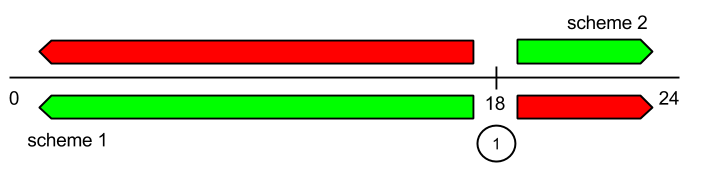
\includegraphics[width=\linewidth]{figures/distance}
      \caption{Distance from intersection points. Positive (green) values indicate the optimal result. Negative (red) represent data for further improvement.}
        \label{fig:distance}
\end{figure}

\begin{algorithm}[H]
 \label{alg:distance_from_optimality}
 \KwData{Uptime, Intersection Point, Bias;}
 \KwResult{Distance from intersection point [-24, 24];}
  \If{Bias} {
        return Uptime - Intersection Point
  } 
  \Else{
        return Intersection Point - Uptime
  }
\caption{Uptime Based Distance From Intersection Points}
\end{algorithm}

Example algorithm results
\begin{enumerate}
\item Input: Uptime: 24, Optimality Point: 18, Bias: True (more optimal for values above threshold). Output: +6
\item Input: Uptime: 16, Optimality Point: 18, Bias: True (more optimal for values above threshold). Output: -2
\item Input: Uptime: 15, Optimality Point: 18, Bias: False (more optimal for values below threshold). Output: +3
\item Input: Uptime: 19, Optimality Point: 18, Bias: False (more optimal for values below threshold). Output: -1
\end{enumerate}

\subsection{Recognize inefficiencies and suggest changes}

\myparagraph{Threshold Based Report}

Generate report of machines based on distance from optimality points. Use customizable threshold. 
Results from the report will be used to calculate suggestions.

\myparagraph{Visual recognition}

Visual recognition as a helper method to define thresholds, especially for further incremental optimizations. 
Useful as static thresholds can miss a whole set of machines that are just below the threshold. 

\begin{figure}[H]
       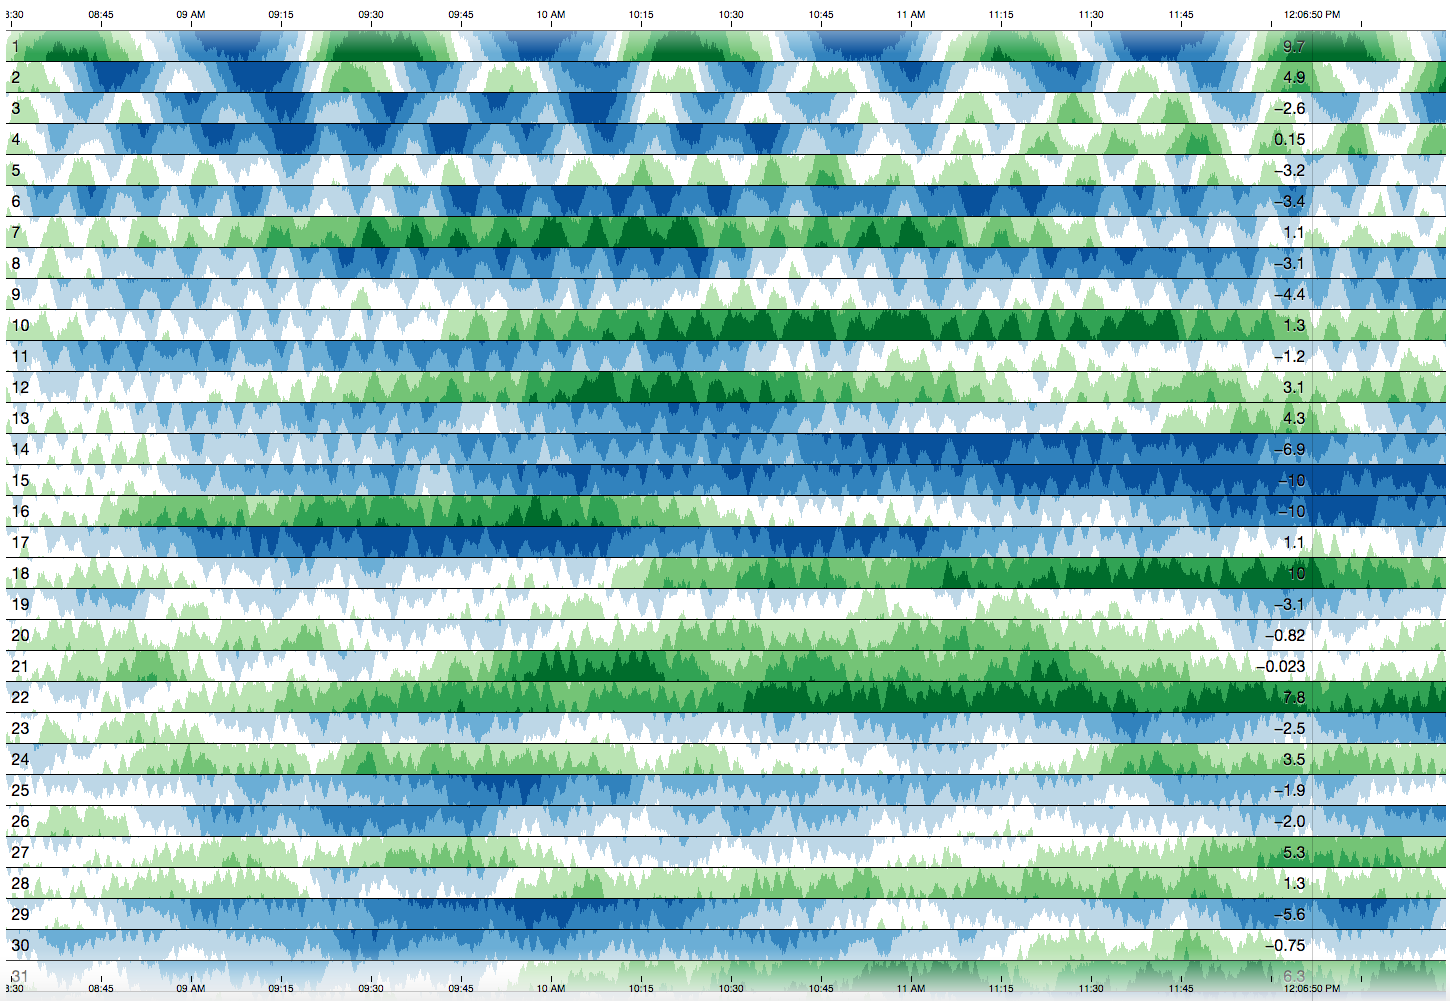
\includegraphics[width=\linewidth]{figures/cubism}
      \caption{Visualization of distance from optimality points. Green - positive, Blue - negative values.}
        \label{fig:cubism}
\end{figure}

\myparagraph{Aggregated CPU and memory usage}

Aggregated values of CPU and memory will help to suggest better utilization strategies that guarantee SLOs. Algorithm~\ref{alg:agg_cpu_mem} represents pseudo-code implementation and~\ref{agg_cpu_mem_implementation} contains implementation in Python with Apache Spark.

\begin{algorithm}[h]
\caption{Aggregated CPU and memory}
\label{alg:agg_cpu_mem}
 \KwData{CPU and memory usage in a form of \textless K, List\textless V\textgreater\textgreater where K is Machine ID}
 \KwResult{Aggregated CPU and memory usage}
 \algrenewcommand\algorithmicfunction{\textbf{class}}
 \algrenewcommand\algorithmicprocedure{\textbf{method}}
  \begin{algorithmic}[1]
        \Procedure{map}{$\textrm{Id } key, \textrm{List } values}$
                \State $\textsc{Emit}(\textrm{Id }key, (cpuUsage, memoryUsage))$
        \EndProcedure
        \Procedure{reduce}{$\textrm{Id } key, \textrm{Int } aggValue}$
                \State $\textsc{Emit}(\textrm{Id }key, a + b)$
        \EndProcedure
  \end{algorithmic}
\end{algorithm}

\begin{minipage}{\linewidth}
\begin{lstlisting}[label={agg_cpu_mem_implementation},caption={Aggregated CPU and memory implementation in Apache Spark},frame=single] 
cpu = distFile.map(lambda(line): 
                (line.split(",")[0], line.split(",")[5]))
            .reduceByKey(lambda a,b: a + b)

mem = distFile.map(lambda(line): 
                (line.split(",")[0], line.split(",")[6]))
            .reduceByKey(lambda a,b: a + b)
\end{lstlisting}
\end{minipage}

\myparagraph{Calculate number of jobs per day}

The number of jobs per day will be a useful parameter to calculate cluster-wide averages used for suggestions. Algorithm~\ref{alg:jobs_per_day} represents pseudo-code implementation and~\ref{jobs_per_day} contains implementation in Python with Apache Spark.

\begin{algorithm}[h]
\caption{Daily jobs count}
\label{alg:jobs_per_day}
 \KwData{Job entry in a form of \textless K, List\textless V\textgreater\textgreater where K is Machine ID}
 \KwResult{Aggregated jobs count}
 \algrenewcommand\algorithmicfunction{\textbf{class}}
 \algrenewcommand\algorithmicprocedure{\textbf{method}}
  \begin{algorithmic}[1]
        \Procedure{map}{$\textrm{Id } key, \textrm{List } values}$
                \State $\textsc{Emit}(\textrm{Id }key, 1)$
        \EndProcedure
        \Procedure{reduce}{$\textrm{Id } key, \textrm{Int } aggValue}$
                \State $\textsc{Emit}(\textrm{Id }key, a + b)$
        \EndProcedure
  \end{algorithmic}
\end{algorithm}

\begin{minipage}{\linewidth}
\begin{lstlisting}[label={jobs_per_day},caption={Aggregated CPU and memory implementation in Apache Spark},frame=single] 
def mapping(line):
    machine_id = line.split(",")[0]
    counter = 1
    return (machine_id, counter)

task_counter = distFile.map(mapping).reduceByKey(add)
\end{lstlisting}
\end{minipage}


\subsubsection{Squeeze-them-in suggestion strategy}

The proposed strategy calculates an amount of spare CPU and memory capacity based on cluster-wide averages. Aggregated value for CPU and memory represents an amount of capacity gathered from machines that are utilized below average. Based on the amount of aggregated capacity, the algorithm will attempt to squeeze in a maximum amount of machines gathered from Threshold Based Report. As a result, it will propose to turn off a number of machines and guarantee that SLOs will be met.
This approach performs well when underutilized machines exist. For well-balanced clusters with similar usage patterns, it does not find a lot of spare capacities and would propose fairly limited improvements. 

\begin{algorithm}[h]
\caption{Squeeze them in suggestion strategy}
\label{alg:squeeze-them-in}
 \KwData{Cluster averages for CPU and memory, List of machines from Threshold Based Report, List of other machines}
 \KwResult{List of machines that can be powered down}
 \algrenewcommand\algorithmicfunction{\textbf{class}}
 \algrenewcommand\algorithmicprocedure{\textbf{method}}

  $float spareCpu = 0;$
  $float spareMemory = 0;$
  $ID[ ] machinesToExclude;$

\ForAll{machine in otherMachines}{
        \If{$machine.cpu < cluster.cpu$} {
                 $spareCpu += clusterCpu - machineCpu$
        }
        \If{$machine.memory < cluster.memory$} {
        	$spareMemory += clusterMemory - machineMemory$
        }
}

\ForAll{machine in machinesFromReport}{
        \If{$(spareCpu - machine.cpu > 0) \&\& (spareMemory - machine.memory > 0)$}{
                add machine to machinesToExclude;
        }
}

\Return machinesToExclude;

\end{algorithm}

\subsubsection{New capacity configuration suggestion}

\begin{algorithm}[h]
\caption{New configuration suggestion}
\label{alg:new_configuration}
 \KwData{List of machines from Threshold Based Report, List of available schemes, Average number tasks per hour;}
 \KwResult{New configuration suggestion}
 \algrenewcommand\algorithmicfunction{\textbf{class}}
 \algrenewcommand\algorithmicprocedure{\textbf{method}}

  $float[ ] totalCost;$
  $float totalCpu = 0;$
  $float totalMemory = 0;$

\ForAll{machine in machinesFromReport}{
        machine.cpu += totalCpu;
        machine.memory += totalMemory;
}

\ForAll{scheme in availableSchemes}{
		hoursPerDay = scheme.getHours();
        cpuCap = hoursPerDay * clusterCpuAvgPerHour;
        memCap = hoursPerDay * memoryCpuAvgPerHour;

        vmsReqCpu = totalCpu / cpuCap;
        vmsReqMem = totalMemory / memCap;

        totalCost[scheme] = min(vmsReqCpu, vmsReqMem) * scheme.cph;
}

\Return{min(totalCost)}

\end{algorithm}



%%%%%%%%%%%%%%%%%%%%%%  
%%% EVALUATION!!!
%%% ALGORITHM TESTING  
%%% ON GOOGLE DATASET 
%%%%%%%%%%%%%%%%%%%%%%

\chapter{Evaluation}

\section{Methodology}

Evaluation process can be splitted into four phases:
\begin{enumerate}
\item collection and transformation of pricing and usage data,
\item calculation of key indicators (\textit{cph, ip(scheme1, scheme2), KDI}) and cluster characteristics (\textit{total cost, performance averages}), 
\item suggestion of changes based on Algorithm~\ref{alg:squeeze-them-in} and~\ref{alg:new_configuration},
\item validation of positive correlation between \textit{KDI} and \textit{total cost} changes.
\end{enumerate}

\section{Setup description}

\myparagraph{Workstation}
Hardware - Intel Xeon 6-core x86\_64 2.4GHz, L3 cache 24MB, RAM 28GB. \\
Operating System - OS X Yosemite 10.10.2

\myparagraph{Platform}
Apache Spark 1.2.1\footnote{\url{https://spark.apache.org}} - an engine for large-scale data processing. All of map reduce jobs were written using Python API. Jobs were executed using standalone cluster mode with settings specified in Table~\ref{tab:spark_conf}. Job run times varied widely based on input data size and complexity of computations - from 20hs+ for transformations on 100G+ data to 1 minute aggregations on 100-200M input.

\begin{table}[h]
\begin{center}
    \begin{tabular}{| l | l |}
    \hline
    \textbf{Setting name} & \textbf{Value} \\
    \hline
    spark.master & local \\
    \hline
    spark.driver.memory & 8G \\
    \hline
    spark.executor.memory & 20G \\
    \hline
    spark.default.parallelism & 500 \\
    \hline
    \end{tabular}
\end{center}
\caption{Apache Spark standalone cluster configuration settings} 
\label{tab:spark_conf}
\end{table}

Settings were tweaked during computation mostly due to frequent Out Of Memory errors. Default driver and executor settings - 256M and 512M respectively - were not enough to handle the volume of input data. Further OOMs occurred during \textit{RRD.reduceByKey}\footnote{\url{https://spark.apache.org/docs/1.2.1/api/python/pyspark.html#pyspark.RDD.reduceByKey}} operations as it required to compute a fairly large hash map. Tweaks of \textit{spark.default.parallelism} setting worked the best as it enforced more granular input data chunking.

\section{Input data}

\myparagraph{Pricing data}

Amazon Web Services\footnote{\url{http://aws.amazon.com/}} offered variable pricing schemes based on uptime. Customer could choose an instance configuration and total cost would be calculated based on a number of hours of uptime per day.
The offering was splitted into three options:
\begin{enumerate}
\item light - low upfront and high per hour cost,
\item medium - medium upfront and medium per hour cost,
\item heavy - high upfront and low per hour cost.
\end{enumerate}

For evaluation purposes we choose two pricing schemes for two different VM configurations~\cite{AWS:light}~\cite{AWS:medium}~\cite{AWS:heavy}. Pricing details are specified in Table~\ref{tab:aws_pricing}

\begin{table}[h]
\begin{center}
    \begin{tabular}{| l | l | l | l |}
    \hline
    \textbf{Name} & \textbf{Scheme} & \textbf{Upfront (\$)} & \textbf{Per hour (\$)} \\
    \hline
    cc2.8xlarge & light & 1762 & 0.904 \\
    \hline
    cc2.8xlarge & medium & 4146 & 0.54 \\
    \hline
    cc2.8xlarge & heavy & 5000 & 0.361 \\
    \hline
    m2.4xlarge & light & 1088 & 0.676 \\
    \hline
    m2.4xlarge & medium & 2604 & 0.52 \\
    \hline
    m2.4xlarge & heavy & 3156 & 0.272 \\
    \hline
    \end{tabular}
\end{center}
\caption{AWS pricing for reserved cc2.8xlarge and m2.4xlarge instances}
\label{tab:aws_pricing}
\end{table}

\myparagraph{Usage data}

Google released 29-day cluster usage traces of more than 12k machines running over 650k jobs~\cite{clusterdata:Reiss2011}. An analysis~\cite{clusterdata:Reiss2012b} revealed that the workload is heterogeneous, which is somewhat unique compared to other traces and makes a good fit for testing.
The trace contains data about jobs submitted by users. Each job is made of tasks. Each task reports metrics about resource consumption - e.g. CPU, memory - and timestamps. The trace does not contain information about the purpose of the jobs, which limits SLO assumptions to resource utilization. 
Resource utilization data is provided in normalized units - the strongest configuration is 1 and the rest of configurations are described in relation to that value.

\myparagraph{Pricing assignment to usage data}

Google trace does not provide any information about pricing schemes of included machines. For evaluation purposes, we will produce example configurations of different pricing schemes that could exist within a real cluster. 

The majority of machines within Google cluster i.e. 82\%, have following configuration: 0.5 CPU, 0.5 RAM or 0.5 CPU, 0.25 RAM. We will assign heavy pricing scheme for these machines. For the rest of the cluster, we will assign medium pricing scheme. 

The light scheme is a good fit for relatively short periods of time, e.g. during peak. An analysis of the trace~\cite{clusterdata:Reiss2012b} shows that jobs with the highest peak-to-mean ratio are production priority jobs and they constitute only 7\% of all jobs. Therefore, we will not assign any light pricing schemes for this evaluation purposes. 

We will refer to cc2.8xlarge and m2.4xlarge reserved instances pricing data as \textit{Scheme 1} and \textit{Scheme 2}.  
 

\section{Input data schema transformation and aggregations}

Google trace data contains a lot of detailed information. This paper focuses on uptime and we extracted only relevant data for further evaluation. Machine and task events original schema is presented on Tables~\ref{tab:machine_events} and~\ref{tab:task_events} and fields selected for further transformation and aggregation are marked in bold text. 

\begin{table}[h]
\begin{center}
    \begin{tabular}{| l | l |}
    \hline
    & \textbf{Column name} \\
    \hline
    1 & \textbf{timestamp}\\
    \hline
    2 & \textbf{machine id} \\
     \hline
    3 & event type\\
     \hline
    4 & platform id\\
     \hline
    5 & \textbf{capacity: CPU}\\
     \hline
    6 & \textbf{capacity: memory}\\
    \hline
    \end{tabular}
\end{center}
\caption{Machine events table schema from Google trace}
\label{tab:machine_events}
\end{table}


\begin{table}[h]
\begin{center}
    \begin{tabular}{| l | l |}
    \hline
    & \textbf{Column name} \\
    \hline
    1 & \textbf{start time of the measurement period}\\
    \hline
    2 & \textbf{end time of the measurement period}\\
     \hline
    3 & job ID\\
     \hline
    4 & task index\\
     \hline
    5 & \textbf{machine ID} \\
     \hline
    6 & mean CPU usage rate \\
    \hline
    7 & \textbf{canonical memory usage}\\
    \hline
    8 & assigned memory usage\\
    \hline
    9 & unmapped page cache memory usage\\
    \hline
    10 & total page cache memory usage\\
    \hline
    11 & maximum memory usage\\
    \hline
    12 & mean disk I/O time\\
    \hline
    13 & mean local disk space used\\
    \hline
    14 & maximum CPU usage\\
    \hline
    15 & maximum disk IO time\\
    \hline
    16 & cycles per instruction (CPI)\\
    \hline
    17 & memory accesses per instruction\\
    \hline
    18 & sample portion\\
    \hline
    19 & aggregation type \\
    \hline    
    20 & \textbf{sampled CPU usage}\\
    \hline
    \end{tabular}
\end{center}
\caption{Task events table schema from Google trace}
\label{tab:task_events}
\end{table}

\begin{table}[h]
\begin{center}
    \begin{tabular}{| l | l |}
    \hline
    & \textbf{Column name} \\
    \hline
    1& machine ID\\
    \hline
    2 & total CPU usage\\
     \hline
    3 & CPU capacity\\
     \hline
    4 & total assigned memory usage\\
     \hline
    5 & memory capacity\\
     \hline
    6 & number of tasks\\
    \hline
    \end{tabular}
\end{center}
\caption{Aggregated statistics from Google trace data}
\label{tab:new_schema}
\end{table}

Table~\ref{tab:new_schema} is a new schema produced from join of capacity metrics from machine events and aggregations computed from tasks events data. 

\myparagraph{Daily usage}
As a first step, the task usage data is grouped into separate buckets to represent 1 day worth of data based on timestamps. Listing~\ref{daily_usage} shows Apache Spark filter implementation in Python. This transformation created 29 folders of data.

\myparagraph{Uptime}
Uptime per day per machine was calculated based on aggregation of task duration times for a given day. Algorithm~\ref{alg:uptime_per_machine} shows design and Listing~\ref{uptime_per_machine_implementation} represents implementation of this aggregation. Total number of hours in cluster is 8705743, which gives 23.36 hours daily per machine on average. 

Transformation to below schema. 
- total number of tasks per day

\myparagraph{Total CPU and memory usage}
CPU and memory aggregation logic is presented in Algorithm~\ref{alg:agg_cpu_mem} and implemented in Listing~\ref{agg_cpu_mem_implementation}. The total CPU consumption of the cluster is 15972217.38, which gives 43.77 daily per machine on average. The total memory usage is 30676363.36, which is 84.06 on average. 

\myparagraph{Total number of tasks}
An aggregated number of tasks is calculated based on Algorithm~\ref{alg:jobs_per_day} and implementation presented in Listing~\ref{jobs_per_day}. The total number of tasks is 1234716525, which gives 3383.65 tasks per day per machine on average.


\section{Pricing data indicators}

\subsection{Cost per hour}

Based on Formula~\ref{eq:cph} implemented in Python and presented on Listing~\ref{cost_per_hour}, we calculated \textit{cost per hour} for both analyzed schemes. Results are presented on Table~\ref{tab:cph:scheme1} and~\ref{tab:cph:scheme2} in respect of number of hours per day a machine would run. The cost per hour drops when uptime per day rises. The same trend exhibits for both schemes.

\myparagraph{Scheme1}
\begin{table}[h]
\begin{center}
    \begin{tabular}{| l | l | l | l |}
    \hline
    \textbf{Hour} & \textbf{Light (price/hour)} & \textbf{Medium (price/hour)} & \textbf{Heavy (price/hour)} \\
    \hline
	1&5.7313972602739724&11.898904109589042&14.059630136986302 \\
    \hline
	2&3.317698630136986&6.2194520547945205&7.21031506849315 \\
    \hline
	3&2.513132420091324&4.326301369863014&4.9272100456621 \\
    \hline
	4&2.110849315068493&3.3797260273972602&3.785657534246575 \\    
	\hline
  5&1.8694794520547946&2.811780821917808&3.1007260273972603 \\
  	\hline
  6&1.7085662100456622&2.433150684931507&2.64410502283105 \\
  	\hline 
  7&1.593628180039139&2.162700587084149&2.317947162426614 \\
  \hline 
  8&1.5074246575342467&1.9598630136986301&2.0733287671232876 \\
  \hline
  9&1.4403774733637749&1.8021004566210044&1.8830700152207003 \\
  \hline
  10&1.3867397260273973&1.6758904109589041&1.73086301369863 \\ 
  \hline
  11&1.342854296388543&1.5726276463262765&1.6063300124533002 \\ 
  \hline
  12&1.3062831050228312&1.4865753424657535&1.5025525114155251 \\
  \hline
  13&1.2753382507903057&1.4137618545837725&1.414740779768177 \\
  \hline
  14&1.2488140900195697&1.3513502935420745&1.3394735812133072 \\
  \hline
  15&1.2258264840182649&1.2972602739726027&1.2742420091324203 \\
  \hline
  16&1.2057123287671234&1.249931506849315&1.2171643835616437 \\
  \hline
  17&1.1879645447219984&1.208170829975826&1.1668017727639 \\
  \hline
  18&1.1721887366818875&1.1710502283105022&1.12203500761035 \\ 
  \hline
  19&1.1580735400144198&1.1378370583994233&1.0819805335255948 \\
  \hline
  20&1.1453698630136988&1.107945205479452&1.045931506849315 \\
  \hline
  21&1.1338760600130462&1.0809001956947162&1.0133157208088714 \\
  \hline
  22&1.1234271481942715&1.0563138231631384&0.9836650062266501 \\
  \hline
  23&1.1138868374032165&1.0338653960690887&0.9565926146515782 \\ 
  \hline
  24&1.1051415525114157&1.0132876712328769&0.9317762557077626 \\ 
    \hline
    \end{tabular}
\end{center}
\caption{cph results for cc2.8xlarge reserved instance}
\label{tab:cph:scheme1}
\end{table}

\myparagraph{Scheme2}

\begin{table}[h]
\begin{center}
    \begin{tabular}{| l | l | l | l |}
    \hline
    \textbf{Hour} & \textbf{Light (price/hour)} & \textbf{Medium (price/hour)} & \textbf{Heavy (price/hour)} \\
    \hline
1&3.656821917808219&7.654246575342467&8.918575342465754\\ 
 \hline 
2&2.1664109589041094&4.087123287671233&4.595287671232876\\ 
 \hline 
3&1.669607305936073&2.898082191780822&3.1541917808219178\\ 
 \hline 
4&1.4212054794520548&2.303561643835616&2.4336438356164383\\ 
 \hline 
5&1.2721643835616436&1.9468493150684931&2.0013150684931507\\ 
 \hline 
6&1.1728036529680366&1.709041095890411&1.713095890410959\\ 
 \hline 
7&1.1018317025440314&1.5391780821917809&1.5072250489236791\\ 
 \hline 
8&1.0486027397260274&1.411780821917808&1.352821917808219\\ 
 \hline 
9&1.0072024353120244&1.3126940639269407&1.2327305936073059\\ 
 \hline 
10&0.9740821917808219&1.2334246575342467&1.1366575342465755\\ 
 \hline 
11&0.9469838107098382&1.1685678704856788&1.058052303860523\\ 
 \hline 
12&0.9244018264840183&1.1145205479452056&0.9925479452054796\\ 
 \hline 
13&0.9052939936775553&1.0687881981032665&0.9371211801896734\\ 
 \hline 
14&0.8889158512720158&1.0295890410958906&0.8896125244618396\\ 
 \hline 
15&0.8747214611872147&0.9956164383561644&0.8484383561643836\\ 
 \hline 
16&0.8623013698630138&0.9658904109589042&0.8124109589041095\\ 
 \hline 
17&0.8513424657534246&0.9396615632554393&0.7806220789685737\\ 
 \hline 
18&0.8416012176560121&0.9163470319634702&0.7523652968036529\\ 
 \hline 
19&0.8328853640951694&0.8954866618601299&0.7270829127613554\\ 
 \hline 
20&0.825041095890411&0.8767123287671232&0.7043287671232877\\ 
 \hline 
21&0.8179439008480104&0.8597260273972603&0.6837416829745597\\ 
 \hline 
22&0.8114919053549191&0.8442839352428394&0.6650261519302615\\ 
 \hline 
23&0.8056009529481835&0.8301846337105421&0.6479380583680763\\ 
 \hline 
24&0.8002009132420091&0.8172602739726028&0.6322739726027398 \\
 \hline 
    \end{tabular}
\end{center}
\caption{cph results for m2.4xlarge reserved instance}
\label{tab:cph:scheme2}
\end{table}

\subsection{Intersection points}

Based on Formula~\ref{alg:intersection points} implemented in Python and presented on Listing~\ref{intersection_points} we calculated \textit{intersection points} between pricing schemes. Table~\ref{tab:intersection_points} shows results of the calculation. Intuitively, heavy schemes is the cheapest option for highly utilized machines. An interesting finding is that medium is never cheaper than light in case of Scheme 2. Figures~\ref{fig:cc2_8xlarge} and~\ref{fig:m2_4xlarge} represent graphically \textit{cph} results and \textit{intersection points} can be noticed.

\begin{table}[h]
\begin{center}
    \begin{tabular}{| l | l | l |}
    \hline
    & \textbf{Scheme 1} & \textbf{Scheme 2} \\
    \hline
    light/medium & 17 & never \\
    \hline
    light/heavy & 16 & 6 \\
    \hline
    medium/heavy & 13 & 14 \\
    \hline
    \end{tabular}
\end{center}
\caption{Intersection points for Scheme 1 and Scheme 2}
\label{tab:intersection_points}
\end{table}

\begin{figure}[H]
  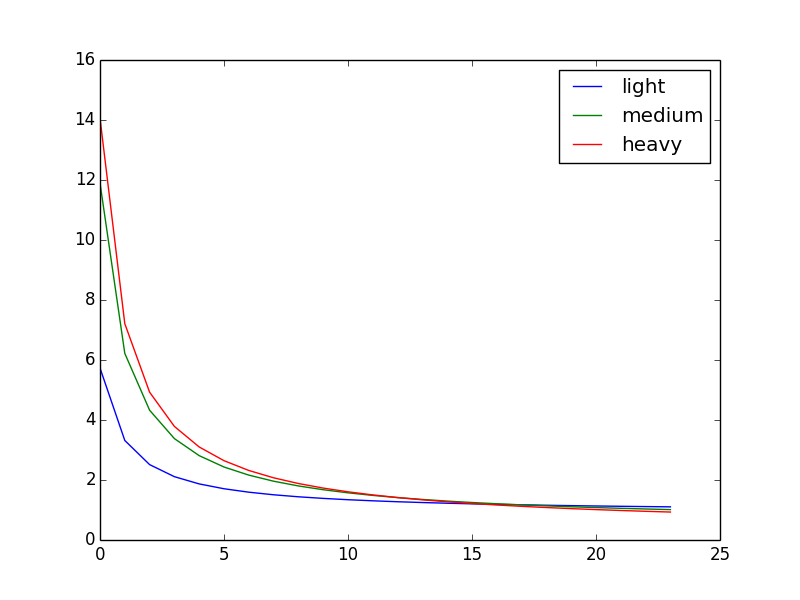
\includegraphics[width=\linewidth]{figures/cc2_8xlarge}
  \caption{\textit{cph} results for Amazon AWS cc2.8xlarge reserved instance rented for 1 year~\cite{AWS:light}~\cite{AWS:medium}~\cite{AWS:heavy}}
  \label{fig:cc2_8xlarge}
\end{figure}

\begin{figure}[H]
  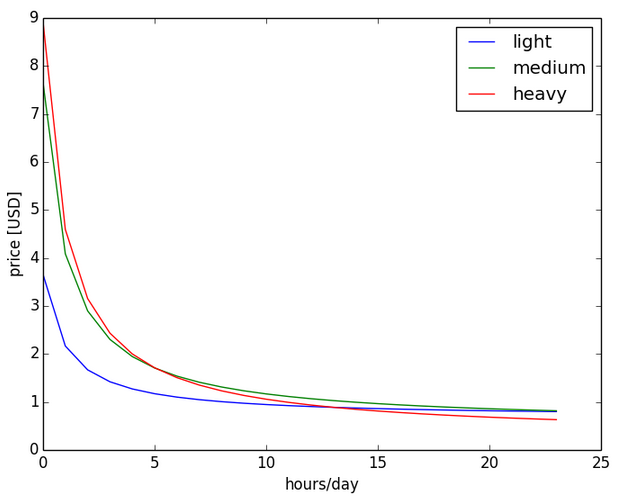
\includegraphics[width=\linewidth]{figures/m2_4xlarge}
  \caption{\textit{cph} results for Amazon AWS m2.4xlarge reserved instance rented for 1 year~\cite{AWS:light}~\cite{AWS:medium}~\cite{AWS:heavy}}
  \label{fig:m2_4xlarge}
\end{figure}

\subsection{Key distance indicator and total cost}

Key distance indicator got calculated for both schemes based on Algorithm~\ref{alg:distance_from_optimality}.

\begin{table}[h]
\begin{center}
    \begin{tabular}{| l | l | l |}
    \hline
    Indicator & Scheme 1 & Scheme 2 \\
    \hline
    Total cost & \$8 177 048 & \$5 637 418 \\
    \hline
    KDI & +3 215 231 & +5 431 137 \\
    \hline
%    Total CPU & 15972217.38 & 15972217.38 \\
%    \hline
%    Total Memory & 30676363.36 & 30676363.36 \\
%    \hline
%    Number of tasks & 1234716525 & 1234716525 \\
%    \hline
    \end{tabular}
\end{center}
\caption{KDI and total cost for cluster}
\label{tab:kdi_and_cost}
\end{table}

\myparagraph{Cluster SLO averages}

Avg cpu usage per machine = 15972217.38/12583 = 1269.35/29 = 43.77
Avg mem usage per machine = 30676363.36/12583 = 2437.92/29 = 84.06
Avg tasks number per machine = 1234716525/12583 = 98125.77/29 = 3383.65


\section{Recognize inefficiencies with Threshold-based Report}

The report will filter all machines that reported non-optimal - negative distance from intersection point - configuration during measurement period (29 days).

\myparagraph{Scheme 1}
Number of machines to tune: 932
CPU capacity to accommodate: 1 320 781.36
Memory capacity to accommodate: 4 286 742.06
Number of tasks to execute: 118869614
Cost of running non-optimal machines: \$657 200
Total uptime: 648519
cost per hour = \$1.01338588383687
Cost per task =  \$657 200 / 118869614 = \$0.00552874681666

\myparagraph{Scheme 2}
Number of machines to tune: 937
CPU capacity to accommodate: 1 327 202.18
Memory capacity to accommodate: 4 303 983.31
Number of tasks to execute: 119367988
Cost of running non-optimal machines: \$532 840.76
Total uptime: 651899


\section{Squeeze-them-in suggestion strategy}

\myparagraph{Scheme 1}
total spare cpu = 3 697 171.44
total spare mem = 6 685 407.83
new KDI: +3 500 037
old KDI: +3 215 231
KDI change: +8.14\%
total uptime = 8056601
new total cost = \$8 177 048 - \$657 200 = \$7 519 848
cost change: -8.04\%
cost per hour = \$7 519 848 / 8056601 = 0.93337723935938
new cost per task = \$7 519 848 / 118869614 = 0.06326131419927

new averages 
cpu per machine = 15972217.38/11651 = 1370.88 / 29 = 47.27 +7.4\%
Avg mem usage per machine = 30676363.36/11651 = 2632.94/29 = 90.79 +7.41\%
Avg tasks number per machine = 1234716525/11651 = 105975.15/29 = +7.4\%

\myparagraph{Scheme 2}
total spare cpu = 3 694 240.56 
total spare mem = 6 682 956.59
new KDI: +5 913 933
old KDI: +5 431 137
KDI change: +8.16\%
total uptime = 8053221
new total cost = \$5 637 418 - \$532 840.76 = \$5 104 577.24
cost change: -9.45\%
cost per hour = \$5 104 577.24 / 8053221 = 0.63385535303204
new cost per task = \$5 104 577.24 / 119367988 = 0.04276336834964

new averages 
cpu per machine = 15972217.38/11646 = 1371.48 / 29 = 47.29 +7.44\%
Avg mem usage per machine = 30676363.36/11646 = 2634.07 / 29 = 90.83 +7.45\%
Avg tasks number per machine = 1234716525/11646 = 106020.65 / 29 = 3655.88 +7.45\%

\section{New capacity configuration suggestion}

vm1 = Entity(c_name, c_light, c_medium, c_heavy)
vm2 = Entity(m_name, m_light, m_medium, m_heavy)

>>> calc_options(uptime, vm2, 29)
(1597, 3727, 972, 567 273.49, 998 186.23, 410 041.68)
>>> calc_options(uptime, vm1, 29)
(1397, 1720, 972, 770 417.58, 876 376.34, 604 274.61)

\section{Validate influence of suggestions and correlation with KDI}

\section{Summary}


%%%%%%%%%%%%%%%%%%%%%%
%%% CONCLUSION AND 
%%% FUTURE WORK
%%%%%%%%%%%%%%%%%%%%%%

\chapter{Conclusion and Future Work}

\myparagraph{Conclusion}
It works and is great!

\myparagraph{Future Work}
\begin{enumerate}
\item Visual recognition of underperforming machines
\item Prediction trend to generate suggestions
\end{enumerate}

%%%%%%%%%%%%%%%%%%%%%%
%%% REFERENCES 
%%%%%%%%%%%%%%%%%%%%%%

\newpage

\label{endpage}
\bibliography{bib}{}
\bibliographystyle{plain}
\end{document}
\end{document}

\end{article}